%% This is file `DEMO-TUDaThesis.tex' version 2.09 (2020/03/13),
%% it is part of
%% TUDa-CI -- Corporate Design for TU Darmstadt
%% ----------------------------------------------------------------------------
%%
%%  Copyright (C) 2018--2020 by Marei Peischl <marei@peitex.de>
%%
%% ============================================================================
%% This work may be distributed and/or modified under the
%% conditions of the LaTeX Project Public License, either version 1.3c
%% of this license or (at your option) any later version.
%% The latest version of this license is in
%% http://www.latex-project.org/lppl.txt
%% and version 1.3c or later is part of all distributions of LaTeX
%% version 2008/05/04 or later.
%%
%% This work has the LPPL maintenance status `maintained'.
%%
%% The Current Maintainers of this work are
%%   Marei Peischl <tuda-ci@peitex.de>
%%   Markus Lazanowski <latex@ce.tu-darmstadt.de>
%%
%% The development respository can be found at
%% https://github.com/tudace/tuda_latex_templates
%% Please use the issue tracker for feedback!
%%
%% ============================================================================
%%
% !TeX program = lualatex
%%

\documentclass[
	ngerman,
	ruledheaders=section,%Ebene bis zu der die Überschriften mit Linien abgetrennt werden, vgl. DEMO-TUDaPub
	class=report,% Basisdokumentenklasse. Wählt die Korrespondierende KOMA-Script Klasse
	thesis={type=bachelor},% Dokumententyp Thesis, für Dissertationen siehe die Demo-Datei DEMO-TUDaPhd
	accentcolor=9c,% Auswahl der Akzentfarbe
	custommargins=true,% Ränder werden mithilfe von typearea automatisch berechnet
	marginpar=false,% Kopfzeile und Fußzeile erstrecken sich nicht über die Randnotizspalte
	%BCOR=5mm,%Bindekorrektur, falls notwendig
	parskip=half-,%Absatzkennzeichnung durch Abstand vgl. KOMA-Sript
	fontsize=11pt,%Basisschriftgröße laut Corporate Design ist mit 9pt häufig zu klein
%	logofile=example-image, %Falls die Logo Dateien nicht vorliegen
]{tudapub}

% Der folgende Block ist nur bei pdfTeX auf Versionen vor April 2018 notwendig
\usepackage{iftex}
\ifPDFTeX
	\usepackage[utf8]{inputenc}%kompatibilität mit TeX Versionen vor April 2018
\fi

%%%%%%%%%%%%%%%%%%%
%Sprachanpassung & Verbesserte Trennregeln
%%%%%%%%%%%%%%%%%%%
\usepackage[main=english, ngerman]{babel}
\usepackage[autostyle]{csquotes}% Anführungszeichen vereinfacht
\usepackage{microtype}


%%%%%%%%%%%%%%%%%%%
%Literaturverzeichnis
%%%%%%%%%%%%%%%%%%%
\usepackage{biblatex}   % Literaturverzeichnis
\addbibresource{research.bib}


%%%%%%%%%%%%%%%%%%%
%Paketvorschläge Tabellen
%%%%%%%%%%%%%%%%%%%
%\usepackage{array}     % Basispaket für Tabellenkonfiguration, wird von den folgenden automatisch geladen
\usepackage{tabularx}   % Tabellen, die sich automatisch der Breite anpassen
%\usepackage{longtable} % Mehrseitige Tabellen
%\usepackage{xltabular} % Mehrseitige Tabellen mit anpassarer Breite
\usepackage{booktabs}   % Verbesserte Möglichkeiten für Tabellenlayout über horizontale Linien
\usepackage{multirow}
\usepackage{hhline}
\usepackage{colortbl}
\usepackage{multicol}
\usepackage{makecell}
\usepackage{xcolor}
\usepackage{listings}

%%%%%%%%%%%%%%%%%%%
%Paketvorschläge Mathematik
%%%%%%%%%%%%%%%%%%%
%\usepackage{mathtools} % erweiterte Fassung von amsmath
%\usepackage{amssymb}   % erweiterter Zeichensatz
%\usepackage{siunitx}   % Einheiten

%Formatierungen für Beispiele in diesem Dokument. Im Allgemeinen nicht notwendig!
\let\file\texttt
\let\code\texttt
\let\tbs\textbackslash

\usepackage{pifont}% Zapf-Dingbats Symbole
\newcommand*{\FeatureTrue}{\ding{52}}
\newcommand*{\FeatureFalse}{\ding{56}}

\begin{document}

\Metadata{
	title=Discriminating if a network flow could have been created from a given sequence of network packets,
	author=Jens Keim
}

\title{Discriminating if a network flow could have been created from a given sequence of network packets}
%\subtitle{subtitle}
\author[J. Keim]{Jens Keim}%optionales Argument ist die Signatur,
\birthplace{Worms}%Geburtsort, bei Dissertationen zwingend notwendig
%FIXME: is Carlos still correct?
\reviewer{Prof. Dr. Max M{\"u}hlh{\"a}user \and Dr. Carlos G. Cordero}%Gutachter

%Diese Felder erden untereinander auf der Titelseite platziert.
%\department ist eine notwendige Angabe, siehe auch dem Abschnitt `Abweichung von den Vorgaben für die Titelseite'
\department{Informatik} % Das Kürzel wird automatisch ersetzt und als Studienfach gewählt, siehe Liste der Kürzel im Dokument.
\institute{Telecooperation}
\group{SPIN}

\submissiondate{\today}
\examdate{\today}

%	\tuprints{urn=1234,printid=12345}
%	\dedication{Für alle, die \TeX{} nutzen.}

\maketitle

\affidavit

\tableofcontents

\chapter{Abstract}

This thesis aims to design a neural network (NN), that is capable of discriminating if a network flow could have been created based on a sequence of packets and can be used as a discriminative network (DN) for a Generative Adversarial Network (GAN) in future work.

For this we first determined the features of network flows and packets a like, which are relevant to this task.
We then created a dataset by extracting the relevant features from well-known network traffic datasets from the field of intrusion detection, as well as falsifying said datapoints to provide negative samples.

For our NN model we compared multiple architectures of recurrent neural networks (RNNs).
Further our model uses a special kind of RNN called a conditional RNN (condRNN) \cite{remyPhilipperemyCondRnn2020}, which already has provided good results for a mixture of conditional and sequential input in the field of image region classification \cite{karpathyDeepVisualSemanticAlignments2015} \cite{vinyalsShowTellNeural2015}.
This is necessary as a flow is the conditional counterpart to a sequence of packets.

% During the phase of testing we optimized dataset and model to be most effective.

\chapter{Introduction}

\section{Motivation}

Network intrusion detection systems (NIDSs) require datasets to be trained and tested.
However, appropriate datasets for NIDSs are hard to come by
since creating authentic synthetic datasets is difficult and time-consuming
and most real traffic is rarely shared due to privacy concerns \cite{ringFlowbasedNetworkTraffic2019a} or copyright \cite{corderoID2TDIYDataset2015}.
This is why researchers in the field of NIDSs are restricted to use datasets with known defects or to create their own datasets.
% Remember that the last sentence of each paragraph should ease the way for the next paragraph.

% Creating synthetic network traffic is essential to provide this kind of datasets.
A researcher that chooses to create their own datasets may use real network traffic, synthetic network traffic, or a mixture of both.
Using real traffic to create a dataset, although desirable, has many disadvantages.
The capture might be too old to represent current networks or
% The network topology recorded, e.g. NAT, % Why is this a problem?
% or the used bandwidth. % not clear what you mean
it may contain artifacts.
Synthetic network traffic is hard to create because network traffic is diverse.
It is influenced by many factors, like
the countless terminals communicating,
the interim devices, e.g. switches, and their bandwidth,
gateways, subnets, and churn of terminals.
To generate appropriate datasets one would need to simulate all those factors and their interactions.
Since this is particularly complicated,
this is where the mixture of real and synthetic traffic comes in.
With this method, one takes an already existing network packet capture and modifies it to fit their needs.
%The idea is good, but the sentence needs work.
% You also need to be carefull and not mix these two ideas:
% 1) Mixing synthetic data with real to create a new dataset.
% 2) Create a complete synthetic dataset from scratch using real traffic as reference.
% Remember that with the GAN technique, we may create completely synthetic traffic that is not mixed with "real" traffic.
This modification can range from adding specific packets, e.g. of an network attack\cite{corderoID2TDIYDataset2015},
to modifying existing packets to fit a new network topology
or altering other significant features of the network behavior by modifying each packet.
Even though this method is quite effective, its design and implementation are also time-consuming and might need to be repeated for each use case.
Since it is difficult to create realistic network packet captures from scratch,
one could propose to create these traffic captures based on network flows, as those are more commonly availabilable.

The paper ''Flow-based Network Traffic Generation using Generative Adversarial Networks'' by Markus Ring et al. \cite{ringFlowbasedNetworkTraffic2019a} provides a method to create synthetic network flows that mimic a given set of network flows.
%This enables researchers to create network flows based on real network flows.
Building on top of this method one could synthetically create labeled datasets of authentic network flows for NIDSs.
However, it is still desirable to have traffic based datasets, since they provide more information than flows.
Instead one could create synthetic network flows like proposed by Ring et al. \cite{ringFlowbasedNetworkTraffic2019a} and
use these already authentic flows to create authentic synthetic network traffic at the packet level.
One approach to this could be a GAN that generates network packet captures based on network flows.

\section{Problem}

If we would want to create a GAN that is able to create the packets from which a network flow was constructed,
three major challenges need to be addressed.
One, the DN of the GAN needs to be defined such that it can determine if a network flow could have been created by a sequence of network packets.
Two, the generative network (GN) of the GAN needs to be able to create network packet captures that are indistinguishable (in some statistical sense) from the packets the network flow was created from.
Three, the training of the GAN and the required datasets.
To create a GAN, both the DN and GN need to perform well on their own.

In this research, we focus on building a NN that can be used as the DN of a GAN in future work.
It is not obvious, however, how to create a DN that
can verify that a network flow was created from a sequence of packets.
This leads to the research questions presented next.

\section{Research Questions}

This thesis will attempt to answer the following research questions.

\begin{itemize}
  \item How can we develop a neural network that acts as a discriminator for a GAN
  that can determine if a network flow could have been created by a sequence of network packets.
  \item Which features of network flows and packets are (most) significant to determine if a network flow could have been created by a sequence of network packets?
  \item Which NN architecture would be most suitable to distinguish if network packets could have created some network flow?
\end{itemize}

\section{Goals and Objectives}

% Was wird bei der Diplomarbeit inhaltlich erwartet und bewertet?

% I picture three main goals for your thesis (you need to either agree or propose something different):
% x 1) Create a dataset (or program to make datasets) to test your theories.
% x 2) Figure out what is needed to distinguish if packets belong to a certain flow, and
% x 3) Come up with an architecture capable of making correct decisions.

This thesis focuses on creating a NN model
that can be used as the DN of a GAN
that takes network flows as input and produces network packets as output.
The NN gets an array of network packets and at least one network flow as input
and provides the probability that a specific network flow was created from the given sequence of packets.
To achieve this goal, we might need to consider additional input,
such as labels for either the network flows, the network packets, or both.
Therefore the goal of this thesis is to create a NN model that distinguishes
if a specific network flow could have been created from a given sequence of packets, or not.

It will not only be necessary to create the NN architecture,
but also the datasets needed to train and test the system.
For this, we need suitable representations of network flows and packets that a NN can process.
To test the reliability of our model, diverse datasets from sufficiently distinct networks need to be constructed.
% During the development of the NN model, these features will be adjusted to create appropriate datasets.
So to reach the goal, we need to reach the following objectives:

\begin{itemize}
  \item Collecting diverse packet captures, representing a wide range of networks.
  \item Extracting flows from said packet captures.
  \item Extracting features from packets and flows alike,
which can be used to distinguish if packets belong to a certain flow.
  \item Creating fake flows by modifying the extracted ones based on those features.
  \item Creating a NN model that is able to compute those features.
  \item Testing the effectiveness of NN architectures to work as discriminators.
  \item Deciding which NN architecture is capable of making correct decisions.
\end{itemize}

%%% THESIS TOPIC END

%\chapter{Requirements}

% Anmerkung von Prof. Mühlhäuser: "Voraussetzungen":
% kann ruhig Selbstverständlichkeiten wie erwünschte Programmierkenntnisse
% beinhalten. Man glaubt nicht, was man bei jedem 10ten (oder so) Diplomanden
% alles irgendwann vermissen wird :-).
% Außerdem kann man "Grundkenntnisse in ... (Themengebiet) wünschenswert
% und förderlich, aber nicht zwingend" hinschreiben, dann kann man
% (z.B. mündlich) argumentieren, dass ein Teil der Literatur vor
% Startschuss zu den 6 Monaten gelesen werden muss.

%\section{for the student}

%\begin{itemize}
%  \item basic familiarity with Python
%  \item basic familiarity with ID2T and Traffic Statistic Extraction
%  \item basic familiarity with yaf and Flow Extraction
%  \item basic familiarity with Tensorflow 2
%  \item basic knowledge of Neural Networks
%  \item broad understanding of RNNs
%\end{itemize}

%\section{for the architecture}

% how much detail?
% regarding the training of GANs/Discriminator
% OR later in Thesis?

%\subsection{Functional Requirements}
% what it should do

%\subsection{Non Functional Requirements}
% how it works

\section{Terminology}
During this work we will use certain phrases and wording that may seem vague but simplifies more complex expressions.

When we say \textit{a sequence of (network) packets belongs to a (network) flow}, we mean that \textit{the (network) flow could have been created from this sequence of (network) packets}.

A \textit{network flow} might also be called \textit{network packet flow}, \textit{packet flow} or just \textit{flow}.

A \textit{network packet capture} might be called \textit{network capture}, \textit{packet capture}, or even \textit{pcap (file)}.

\chapter{Background}

% In every background "item", always start stating why the topic is important to know in the context of your thesis.

%\section{Network intrusion detection systems}
%To understand the motivation behind this thesis we must understand how NIDSs work.
%Intrusion detection systems (IDSs) describe hard- or software that monitors a network or system for malicious activity or policy violations.
%One differentiates between NIDSs and host-based intrusion detection systems (HIDSs).
%The former monitor a network, while the later a single system.
%
%Today NIDSs are crucial for network security.
%Therefore we focus on them.
%There are two different classifications of NIDSs:
%signature-based NIDSs and anomaly-based NIDSs.
%Signature-based systems are limited for several reasons:
%the availability of signatures,
%the growing threat of federated attacks that split the malicious signature between multiple gateways.
%
%This is where anomaly-based detection comes in.
%They classify network behavior as either normal or anomalous.
%This way even new attacks, for which no signature is yet provided,
%can be recognized by the system, since it is anomalous to the network behavior it knows about.
%These systems have two main sources of knowledge:
%the network they observe all the time
%and the datasets they get trained with.

\section{Network Flows v.s. Network Packets}

If we want to extract features from network flows
we first need to understand the difference between network flows and network traffic captures.
A network packet capture is a recording of network traffic at the packet level.
It is limited by a start and end time.
Each packet within the capture contains all header information it contained during actual transmission.
The payload of the packets is omitted if its size gets too large to be reasonably stored otherwise, the packets are unaltered.
A network flow on the other hand is an artificial logical equivalent to only one network connection \cite{brownleeTrafficFlowMeasurement}.

This connection may be between two terminals, a multicast group or a terminal and a broadcast address \cite{rajahalmeIPv6FlowLabel}.
Like a network packet capture, a flow is limited by a start and end time,
but it does not contain information on individual packets.
It holds aggregated information of the network packets within the connection.
For a packet to classify as belonging to a flow the packets typically need to share properties like transport protocol, source and destination IP as well as source and destination port \cite{FlowbasedNetworkTraffic} \cite{claiseSpecificationIPFlow}.
So it describes the connection on a more abstract level and provides less information than a network packet capture.

For example a flow in the YAF format will only keep track of a minimum of header information, like source and destination IP address and port.
It will contain the flags used by the first and last packet of the communication,
but it will not contain the flags of each individual packet within the communication.
It will know the duration and average round trip time of the communicating, but not the time intervals between two packets.
Additionally it might have information the packets themselves do not provide, e.g. the reason for the end of the communication \cite{YAFDocumentation}.

%  aggregation of transmitted network packets  which share some properties [16].
% Typically, all transmitted network packets with the same source IP address, source port, destination IP address, destination port and transport protocol within a time window are aggregated into one flow.
% NetFlow [15] aggregates all network packets which share these five properties into one flow until an active or inactive timeout is reached. In order to consolidate contiguous streams the aggregation of network packets stops if no further packet is received within a time window of α second (inactive timeout).
% The active timeout stops the aggregation of network packets after β seconds, even if further network packets are observed to avoid unlikely long entries.

\subsection{YAF}

Yet Another Flowmeter (YAF) is a tool to create network flows based on network traffic.
It is capable of saving bidirectional flow data of an active link or extracting flows from an offline capture file.
It uses IPFIX-based data structures and file formats, which can also be exported and used by IPFIX compliant toolchains.
We will use the later functionality will help us to create a dataset for our use case.
With \lstinline{yafscii} YAF provides a tool to export YAF network flow data as plain text.
This will also come in handy for us, as we try to keep our dataset sampling simple by using csv files.

\subsection{Wireshark}

Wireshark is probably the most well-known network traffic tool out there.
It is capable of capturing, displaying, sorting and filtering network traffic captures, as well as analysing network packet captures.
It also has other fucntionality, but we mainly use the filter functionality.
It comes with a GUI but also provides a CLI tool called \lstinline{tshark} that is theoretically capable of doing everything the GUI does, just a bit quicker.
This is what we will use.

\section{Network traffic datasets}

This thesis aims to lay the groundwork for a new method of the creation of authentic synthetic network packet captures
that can be used for labeled datasets for training and testing NIDSs.
Anomaly-based NIDSs (ANIDS) need network traffic datasets for testing and training.
Those datasets need to be appropriate to the threat and labeled accordingly.
However appropriate datasets are hard to come by.
Most real traffic recordings are rarely shared due to privacy concerns \cite{ringFlowbasedNetworkTraffic2019a} or copyright \cite{corderoID2TDIYDataset2015}.
The datasets including network attacks,
which are shared publicly,
tend to either be snapshots from real attacks or synthetically created traces from an isolated network.
The later does not provide realistic non-attack traffic, or background traffic.
The former present the problem of non-attack traffic being of a unique network in a unique time frame and therefore not representative of every network.
Also, they most likely get anonymized and are therefore do not represent the ground truth.
Thus these datasets are not sufficient to train or test NIDS.
And no matter the origin the dataset will only describe the network and the behavior of its traffic at the time of recording or creation, hence it might not be applicable in future networks \cite{ringFlowbasedNetworkTraffic2019a}.

% packets > flow - possible
% flow > packets - not possible yet

% NN, decision making, sequential (network) data

\section{Neural Networks}

\subsection{Recurrent Neural Networks}

To solve the problem stated in this thesis we are required to find an appropriate NN architecture.
Our NN model should be able to decide if a network flow could have been created from a sequence of network packets.
The most commonly used NN architecture for sequential data are recurrent neural networks (RNNs).
A feed-forward NN usually processes each input independently from previous inputs.
RNNs store a hidden state obtained from the previous result of the NN and uses them to process the next input.
Natural language processing usually benefits from this, as this allows to draw connections between the words within a sequence.
In theory, this ''memory'' can hold information about all previous calculations,
but in practice, it can only keep track of the last few steps.
This is due to the vanishing gradient problem \cite{hochreiterLongShortTermMemory1997}.

\subsubsection{Vanishing Gradient Problem}

The vanishing gradient problem describes an RNNs tendency to forget earlier timestamps of a longer sequence.
It is also known as the short term memory problem.
To understand how this problem manifests one needs to understand how an RNN operates.
To ensure a single big value within one timestamp does not make other values less significant, but also do not lose their relation to each other, RNNs use the hyperbolic tangent function to ensure the values stay between -1 and 1.
The values in the middle of the range of data are now closest to 0.
However this also means that those values become so small that they do not contribute to the learning process of the RNN anymore.
Thus vanishing from the weights.

\subsection{Long Short Term Memory \& Gated Recurrent Units}

This is where Long Short Term Memory (LSTM) networks \cite{hochreiterLongShortTermMemory1997} or Gated Recurrent Units (GRUs), formerly known as gated recursive convolutional neural network (grConv) \cite{bahdanauNeuralMachineTranslation2016}, come in.
Both similarly tackle the short-term memory issue,
also known as the vanishing gradient problem \cite{hochreiterLongShortTermMemory1997}.
Where the weight of the memory is changed so little, that it becomes insignificant.
Both models provide a gated approach.
They also both rely on the sigmoid function in addition to the hyperbolic tangent function a simple RNN (SimpleRNN) uses.
While the hyperbolic tangent function produces values between -1 and 1,
the sigmoid function produces values from 0 to 1.
This benefits the memory since low impact data is multiplied by 0 and therefore left out of the equation.
If the value is multiplied by 1 it stays the same.
So the internal gates help the NN to learn what data is important and what data can be forgotten, while keeping the important data in memory.
The difference between LSTMs and GRUs lies in how they use the sigmoid function in their internal gates.
%, see figure \ref{fig:LSTMvGRU}.

LSTMs have three gates, the forget gate, the input gate and the output gate, and two states, the cell state and the hidden states. \cite{phiIllustratedGuideLSTM2020}
The forget gate performs a sigmoid operation on the previous hidden state and the current input.
The result is than used as a multiplier for the cell state, effectively letting the NN forget any information that is no longer relevant after taking the new input into account.
The input gate gets the same input, but uses the hyperbolic tangent and sigmoid functions in parallel and than multiplies their results.
The sigmoid function helps to decide which of the current data, provided by the hyperbolic tangent function, is important to keep, as this result will be added to the cell state.
The output gate decides what information the next hidden state should carry.
It calculates the sigmoid function on the concatenation of the previous hidden state and the current input, just as the other gates.
The results gets used as weights for a hyperbolic tangent operation on the new cell state, meaning simple multiplication.
The newly calculated cell state and hidden state get passed to the next timestamp.

GRUs have only two gates, the reset gate, and the update gate, and the cell state. \cite{phiIllustratedGuideLSTM2020}
%In short the update gate combines the forget and update gate of a LSTM, while the reset gate provides the functionality of the LSTMs output gate.
The update gate uses a sigmoid activation over the current input and the previous cell state, as the GRU has no hidden state.
The inverted values are than used to weight the cell state.
% explain why? NO, does not matter
The reset gate again uses the same sigmoid unit and data as the update gate.
This result gets multiplied with the current cell state and concatenated with the current input.
This concatenation is processed by a hyperbolic tangent and multiplied by the non-inverted values of the update gate, before being added to the current cell state.
A GRU has less activations than a LSTM and thererfore requires less computation.
This is illustrated in the schematic comparison in figure \ref{fig:LSTMvGRU}.

Now we have seen how different RNNs operate and how LSTMs and GRUs solve the vanishing gradient problem for sequential input.
In our case however, we do provide more than one input and not all of our inputs are sequential.

\begin{figure}
    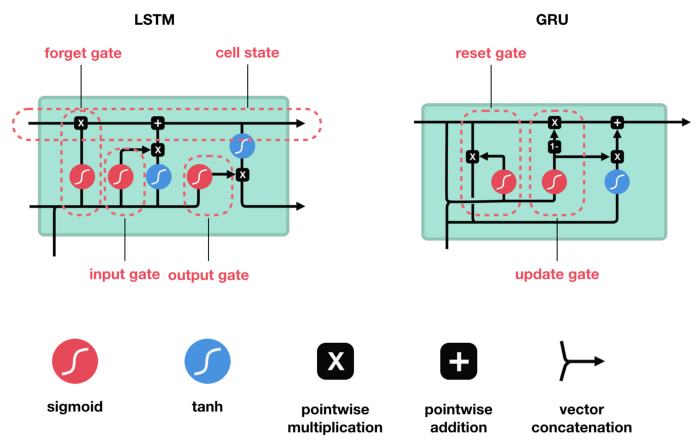
\includegraphics[width=\textwidth]{LSTMvGRU.png}
    \caption{Schematic comparison of LSTMs and GRUs, created by Micheal Phi \cite{phiIllustratedGuideLSTM2020}}
    \label{fig:LSTMvGRU}
\end{figure}

% RNN
% new cell state = tanh(input + previous cell state)

% LSTM
% new cell state = (previous cell state * forget gate) + input gate
% new hidden state = output gate * tanh(new cell state)
% gates:
% \begin{itemize}
%   \item forget gate: sigmoid(input + previous hidden state)
%   \item input gate: sigmoid(input + previous hidden state) * tanh(input + previous hidden state)
%   \item output gate: sigmoid(input + previous hidden state)
% \end{itemize}

% GRU
% new cell state = (previous cell state * update gate) + output gate
% gates:
% \begin{itemize}
%   \item reset gate: sigmoid(input + previous cell state) * previous cell state
%   \item update gate: 1 - sigmoid(input + previous cell state)
%   \item ''output gate'': tanh(input + reset gate) * sigmoid(input + previous cell state)
% \end{itemize}

\subsection{Conditional Recurrent Neural Network}

% TODO
This is where the conditional recurrent neural network (condRNN) comes in.
Compared to the earlier explained RNN, it allows a second input, a conditional input.
Just what we need for our flow data.
The conditional input gets used to set the initial state of the RNN for each datapoint.
% TODO: explain how the initial state is set
This allows the conditional data to be taken into account without appending it to each timestamp in the sequence.

\subsection{GANs}

To create a NN that could later be used as a DN we first need to understand how a GAN operates.
A GAN consists of two NNs that compete against each other to maximize the quality of the generated data:
a generator network (GN) and a discriminative network (DN).
The GN is constantly trying to fool the DN with data it generates synthetically,
while the DN is constantly trying to figure out if the data it was given is real or synthetic.
If correctly optimized, a GAN may create synthetic data indistinguishable from real data.
% TODO: more

\chapter{Related Work}

\section{Flow-based Network Traffic Generation using Generative Adversarial Networks}

Ring et al. \cite{ringFlowbasedNetworkTraffic2019a} introduce a GAN to generate synthetic network flows.
Not only are their synthetically created network flows interesting as the source of input for the proposed GAN in future work,
their choice and classification of network flow features might be valuable resource for this thesis.
% TODO: explain more?
They classify transport protocol, IP addresses and ports as categorical features, duration as continuous, the number of bytes, and packets as numeric.
TCP Flags could either by seen as binary attributes or one categorical value.
Even though Ring et al. \cite{ringFlowbasedNetworkTraffic2019a} do not create network packet captures, most of their classification is applicable to our problem.
In addition they reference and apply a novel approach for the conversion of categorical features of network flows.
They call it IP2Vec.

\subsection{IP2Vec}

Network flows consist of multiple features, some of which are categorical, e.g. IP addresses, ports, and protocols.
However, NNs work best with continuous and numerical data.
To effectively train a NN we, therefore, need to represent those categorical features as numerical data.
For this we planned on using IP2Vec proposed by Ring et al. \cite{ringIP2VecLearningSimilarities2017}.
This solution produces similarity values for IP addresses based on the behavior of the host.

They based their work on the concept of word2Vec from the field of natural language processing.
There the word is observed in the context of its neighbors instead of alone.
Similarly, in IP2Vec IPs are not observed on their own, but on in the context of other features they correlate with.
But instead of words IP2Vec processes network flow attributes,
specifically source IP, destination IP, destination port and protocol.
However one could change those attributes and determine the difference between IPs based on different attributes.
With this approach they are able to determine the differences between IPs based on their communication patterns (aka similar behavior).
For example, a destination IP that correlates with port 80 often can be easily classified as an HTTP server.
Their experiments show that provided the right dataset, the data produced by IP2Vec can be used to distinguish between infected and non-infected hosts, as well as between servers, clients and even printers.

\subsubsection{Conclusion on IP2Vec}

% We had planned to adapt the IP2Vec approach and extend it to handle not only flow attributes but all packet header attributes.
% However since this approach seems fundamentally flawed.

% used IP2Vec to generate source IP based vectors that represent the similarity between IP addresses within a dataset.

% Out of the YAF flow features the following are used by IP2Vec:
% Duration, protocol, source IP, source port, destination IP, destination port, packet count (forward), octet/byte count (forward)

After due consideration, we decided not to use the IP2Vec approach.
This is mainly to the fact that IPs do not influence the flow behavior too much.
The only feature of them that influences a flow significantly is if they are public or local (aka private).
Additionally, IP2Vec sees IPs in the context of a series of packet flows, which represent a network traffic capture,
meaning that it relates the IPs to one another depending on the behavior of their flows within one network.

This is not applicable to our use case, since we use the traffic of multiple network packet capture datasets.
To use IP2Vec we would either have to apply it before extracting the flows and mixing the results,
or mix the flows and then apply IP2Vec to it.
The former bares two problems:
Firstly we would risk introducing false correlations between IPs from different datasets.
As an IP address could appear in more than one network capture and have completely different behavior.
Mixing the information IP2Vec extracted from both of the captures would distort the results of the NN regarding the affected flows.
Secondly we would assume that for our GAN in the future work, we have a whole set of flows for each IP address, that could provide the data necessary to apply IP2Vec before using the flow as input to the DN.
This will most likely not be the case, as we the GN of the GAN would try to create a sequence of packets based on the input of one flow.
% FIXME: is this really the problem? THINK ABOUT IT
The later IP2Vec approach has the problem, that IPs will correlated to each other without ever having been in the same network.
IP2Vec does not account for problems that might result from this.
The best-case scenario is that two IPs from different captures will be classified as being unknown to each other.
But even this holds the issue that a later flow may have communication between those IP addresses and the GAN will have problems generating packet data that will satisfy the DN, because to the DN this will look like an anomaly.
Both approaches have the problem of IPs that might be present in multiple source datasets.

\section{Related Neural Network Models}

In addition, we researched related work regarding NNs, RNNs and GANs, specifically DNs.
Since some approaches to solutions for other problems might be applicable to our problem.
The discrimination if a network flow could have been created from a given sequence of network packets.
This will become clearer once the feature sets of network flows and packets are defined.

% Approaches to generate synthetic network packets that did not use NNs are not really related work,
% since they will not face the same problems as this thesis, therefore they were omitted.

% Bidirectional RNN?

\subsection{Image description generation}

On first glance the field of image description may look out of the scope of this thesis.
However in computer science and machine learning in particular, it is not unlikely for two very separate problems to have the same solution.
The process of teaching a NN to describe an image or even different regions of the image using natural language is a big and complex problem.
The papers "Show and Tell: A Neural Image Caption Generator" by Vinyals et al. \cite{vinyalsShowTellNeural2015} and "Deep Visual-Semantic Alignments for Generating Image Descriptions" by Karpathy and Fei-Fei \cite{karpathyDeepVisualSemanticAlignments2015} both solve this problem in 2015.
However the problem we were interested in is much smaller.

How did both Vinyals and Karpathy solve the problem of multiple inputs for RNNs?
They had the image data and the descriptions in natural language.
While the sequence of descriptions is sequential the image data is not, but it still needed to be included as input for the RNN.
This is where both parties simultaneously create a condRNN, that took the image as conditional input in the beginning and the descriptions as sequential input.
The conditional input conditions the state of the RNN before the sequence is read.
% TODO: explain the conditional RNN better

\subsubsection{Deep Visual-Semantic Alignments for Generating Image Descriptions} % Karpathy

Karpathy et al. extract pixel data of the whole image and the 19 locations within the image.
%, extracted by their region convolutional neural network (RCNN).
They use a convolutional neural network (CNN) to convert each set of pixels into a vector of h dimensions.
%, where h is the number of inputs of the RNN.
So each image is represented by a set of 20 vectors with h dimensions.

300-dimensional word2vec

\subsubsection{Show and Tell: A Neural Image Caption Generator} % Vinyals

Vinyals et al. also use a CNN to create a proper representation of the image that can be passed to the RNN.
For the RNN they chose the LSTM model

% TODO: search and add some more GANs network flow papers

\chapter{Approach}

\section{Methodology}

For our NN model, we assume that some form of Recurrent Neural Network (RNN) will be suitable as a discriminator of a GAN that can create synthetic network packet captures from network flows.
Since simple RNNs have the problem of short-term memory, we propose the use of either Long Short Term Memory (LSTM) networks \cite{hochreiterLongShortTermMemory1997} or Gated Recurrent Units (GRUs) \cite{bahdanauNeuralMachineTranslation2016}.
GRUs tend to use fewer operations and states to produce similar or better results than LSTMs.
But depending on the use case, LSTMs might still produce better results.
It is to be determined, which of the two neural networks provides better results for the problem in this thesis.

For this we will run experiments with the \textbf{SimpleRNN}, \textbf{LSTM} and \textbf{GRU} layers provided in Tensorflow.
\textbf{SimpleRNN} will provide the baseline for the real contenders \textbf{LSTM} and \textbf{GRU} during the experiments, as it will most likely provide the least optimal results.
Before we can pursue the experiments however we need data to train an test with.

% TODO: what is the baseline for the datasets?

\section{Dataset}

For our dataset we will extract packet sequences from publicly available and well-known network packet captures and create network flows based on these sequences.
Each network packet sequence will be paired with its network flow so that our NN can learn the connection between the two data structures.
Since the end goal in the future work GAN is to generate the complete packet sequences based of the flows,
each sequence of packet features will contain as much of the original header information as needed to reconstruct a packet sequence from them.
This way, no crucial information gets lost and the DN is prepared to handle whole packet captures and compare them to flows.

Each header attribute is converted into an appropriate representation depending on its data type and meaning.
Since the NNs are most efficient with continuous and numerical data, we will convert all fields accordingly, whereever possible.
We will also implement a way to create negative samples from the ground truth, which builds our positive samples.
Both will be discussed further in the dataset preprocessing section.

\subsection{Dataset Preparation}

The NN needs to be trained with a significant amount of data, both positive and negative datapoints so that it can make informed decisions.
This will be provided in two steps.
First we sample flows from multiple packet captures we extracted from popular intrusion detection datasets with network traffic packets.
Those samples represent the ground truth and will be our positive datapoints.
Later we randomly apply modifications to those samples to create negative datapoints.

\subsubsection{Sampling}

% FIXME: one capture each might be bad (sound bad)
Instead of combining all flows from our source captures, we sample sequences of packets from only one packet capture of each dataset.
The sampled packet sequences and flows are stored separately as csv files for further preprocessing, as network packet captures are usually slow to process.
For our purpose we considered two approaches for sampling a network packet capture for flows.
Either by sampling through the packet sequences within the captures or by splitting the capture into intervals and sampling through those partial captures.
Splitting the capture into intervals is less compute-heavy and therefore time-intensive, since the resulting packet captures are smaller and much quicker to parse.
Truncated flows should not be a problem, since a capture itself is truncated at beginning and end anyway.
Additionally we also do not need any flow longer than the intervals themselves,
as we use timeouts for the flow collecting.
Later in the preprocessing we also drop any flow longer than 500 packets, to ensure a maximum length and therefore an equal length for the packet sequences.

The question however is the length of the intervals.
Should they be determined relative to the size of the capture or should they have a fixed length?
A fixed-length may provide better comparability between the flows of different captures,
but the variation between packet captures regarding packet rate (frequency) may proof to be problematic.
As setting the fixed length to low may yield the problem that some captures return empty intervals
and setting it too high might result in too large intervals and therefore partial captures to be efficiently parsed later on.
An interval length based on the percentage of each individual capture does not have those faults.
Even though it might shrink the flow duration of smaller captures, it appears to be the better approach.
In addition, extracting packet sequences with a relative offset within a capture might provide sequences with a wider range of flow behavior.

Now that we know we want to split the capture first, it is to be decided, how we sample the packet sequences within an interval.
We can make an educated guess that randomly selected samples will yield better results than sequential sampling, as it again provides a wider range of flow behavior.
Still the degree to which the sampling is randomized should be determined.
% FIXME: drop everything below here?
Do we pick random intervals, or do we pick the sequence of packets within each interval at random.
Do we pick every 20th packet sequence, or do we pick each packet sequence at random.
We might test a variety of those methods to choose the packet sequences, when improving the dataset, once we have some results from the NN.
% to here

For the first iteration of our dataset we decided, that splitting the capture into intervals first would be the right approach.
We split the captures into intervals relative to its size.
This way we will preserve the behavior of the sampled flows within the larger network within each specific interval.
Afterwards, we will randomly sample up to 250 of TCP and UDP packet sequences alike within those intervals.
% TODO: mention that not all sources provide "enough" flows per protocol, specifically UDP

Each sampled packet sequence will be exported as a capture first.
The header fields of the packets belonging to the sequence will be stored as a csv file for easier parsing.
Then we use YAF to extract the flow information and yafscii to create flow-based csv files form the exported capture.

\subsubsection{A Padding supported Conversion from UDP to TCP}

Each datapoint in our dataset can either be a TCP or a UDP packet.
Compared to UDP packets, TCP packets have much more header fields and therefore more (derived) features.
This results in an uneven timestamp size (length of packet entries) between datapoints, if one is based on a UDP packet and one is a TCP packet.
To make packets of both protocols comparable, we will add padding to the UDP packets.
We add the TCP flags and options as well as the sequence number and window size with a masking value (-15) , more on that in the model section.
To round it up we convert the UDP length to TCP header length and TCP payload length, see Dataset Criteria paragraph derivation.
The last part is especially important to keep the datapoints comparable.
This way, the NN can make the right decisions based on the data.

\subsubsection{Creation of negative samples}

To create negative samples we use multiple different methods.
The first is falsifying packet and flow features by either sampling them from another datapoint of the dataset or generating random values, which lie within a rough frame of expectation for the feature.
Both processes are randomized.
And both produce three different types of negative samples:

\begin{itemize}
    \item a datapoint, which has modified (falsified) packets
    \item a datapoint, which has a modified (falsified) flow
    \item a datapoint, which has both
\end{itemize}

% double check, but this actually makes sense
We decided not to alter the flow as the RNN should learn if a packet sequence could have been created by a given flow.
In this scenario the flow is authentic and does not need to be classified itself for authenticity.

The second method is randomizing the packet order within the packet sequence of a given datapoint.
The third is to decrease or increase the number of packets of a sequence in a given datapoint.
To decrease the number of packets we just remove a random number of packets at a random position.
To increase the number of packets we again sample from another datapoint in the dataset and add some of its packets to the current sequence.
And the fourth and final method is mismatching network flows with a different sequence of packets.

This procedure provides us with a wide range of negative datapoints.
This is important in order to efficiently train the NN.
However it is important to falsify the data in a realistic way, so that the NN is efficiently tested for the future use within a GAN.
For this we need to provide a good representation for each feature of packets and flows.

\subsection{Dataset Criteria}

In this section we discuss, which features will be part of our dataset and how they need to be derived to function as input for the NN.
All network traffic features influencing network flow behavior will be of importance to our NN.
This will therefore decide the criteria of the dataset features.
Network flows and packet captures of packet sequences will be the source of our datapoints.

% FIXME: move this UP?
We will generally focus only on IPv4 traffic to keep it simple.
Also we will focus on the TCP and UDP protocols for now.

% Network flows created by YAF contain the following features:
% % start-time, end-time, duration, rtt, proto, sip, sp, dip, dp, iflags, uflags, riflags, ruflags, isn, risn, tag, rtag, pkt, oct, rpkt, roct, end-reason
% Timestamps for start and end time, duration, round trip time, protocol, source IP, source port, destination IP, destination port, TCP flags (forward and reverse), initial TCP sequence number (forward and reverse), first-packet 802.1q VLAN tag (forward and reverse), packet count (forward and reverse), octet/byte count (forward and reverse), the reason for the end of the packet sequence.

\subsubsection{Packet sequence features}

\definecolor{not}{HTML}{949698} % Gray
\definecolor{trivial}{HTML}{ed1b23} % Red
\definecolor{derivation}{HTML}{fff200} % Yellow
\definecolor{feature}{HTML}{41b0e4} % CornflowerBlue
\definecolor{dropped}{HTML}{99479b} % purple

Each packet contains a variety of header fields depending on its protocol and the options chosen by the communicating end points.
It is to be decided, which of those header fields are of importance to our goals.
If we just wanted to validate that a sequence of packets belongs to a flow, we could argue that the only header fields interesting are the ones that are present in the flow representation as well.
But for the future work GAN this would not be enough.
Instead we want our NN to learn the correlation between all packet header fields and the flow features.
This will enable the NN to be used as a DN for the proposed GAN later.

One could argue that to properly correlate between flows and packets we need all of the header fields of each packet.
%Ideally all of them, but some can be ignored and others simplified for the NN.
However most of the header fields can be trivially verified by directly comparing to the flow features (addresses), order checking (acknowledgement numbers) or similar methods.
% FIXME: wording
For this reason some header fields are insubstantial for our use case, for example the addresses of the communicating end points (source and destination).
This includes MAC and IP addresses.
Tables \ref{mac} to \ref{udp} present an overview of the packet headers and their fields.
We color code packet header fields in five categories:
\colorbox{not}{\textbf{{Not Used}} (gray)},
useful but \colorbox{trivial}{\textbf{Trivial} (red)},
\colorbox{dropped}{\textbf{Dropped} (purple)},
\colorbox{derivation}{\textbf{Feature Derivations} (yellow)},
and raw \colorbox{feature}{\textbf{Features} (blue)}.

\paragraph{\colorbox{not}{\textbf{{Not Used} (gray)}}} are header fields that do not change ever or at least not in our scenario.
This includes the Version of the IP Header, since we only take IPv4 traffic into account,
and the reserved bits in the IP flags and the TCP header.

\paragraph{\colorbox{trivial}{\textbf{Trivial} (red)}} header fields might be useful, but should not be fed to the NN.
Either because they can easily be checked/validated outside the NN and might slow the NN down for no benefit.
Or they do not alter the behavior of the network flow.
% TODO QUESTION: what about IP class? this could be an interesting feature
% No, but difference between public and local.
This would include header lengths, urgent pointer, as well as MAC and IP addresses.
% FIXME: header lengths
The acknowledgement number order can be easily checked outside the NN and can be omitted as well.

\paragraph{\colorbox{dropped}{\textbf{Dropped} (purple)}} fields could have been \colorbox{derivation}{\textbf{Feature Derivations} (yellow)}, but were omitted due to a lack of data.
A NN needs a large amount of data to make proper decisions, if the data is not sufficient and it encounters a feature for the first time it would at best classify the datapoint correctly with a 50\% chance.
Without sufficient data, we can not train our NN and they would just be a dead feature.
For IP options and the TCP flag NS, also called the ECN-nonce, the data is inconclusive,
as our dataset does not contain any flows with IP options and only three with the NS flag set.
This however is not unusual, as those fields are rarely used in practice anyway.
Since our dataset is constructed from numerous network packet captures from statistically different intrusion detection datasets,
it supports our research results that this is indeed just normal network traffic behavior.
Luckily network flows do not contain either of those features, meaning it should not impact our results.
IP options would influence the behavior of a flow, but as our dataset does not contain any IP options, omitting them does not result in bad training results.
It only means that in order to take IP options into account in the future our NN and preprocessing needs to be expanded.
The ECN-nonce is the more acute problem since less than 0.0009\% of datapoints use it. % FIXME: double check this number?
Which would add an additional risk for our NN to misinterpret the data, once it comes accross such a datapoint.
Omitting the ECN-nonce however should not be a problem, as the feature does not impact the behavior of the flow in any way that is not already indicated by the ECN value, see later in this section.

\paragraph{\colorbox{derivation}{\textbf{Feature Derivations} (yellow)}} are fields, which can not be used as direct input to the NN,
but need to be derived in some way beforehand.
The raw data representation of those features is not optimal as NN input and needs to be abstracted in a certain way.
The most prominent feature type is the categorical feature, but simple byte or string conversion can also already qualify for this category.
The type of derivation can vary from header field to header field.
The protocol for example will be represented as a single boolean as our dataset only contains TCP and UDP, where 1 stands for TCP and 0 for UDP.
Take note that UDP length, which describes the total length of the UDP frame, will be derived to TCP length, a wireshark filter describing the payload size of TCP packets, and the data offest, which is equivalent to the TCP header length.
This way packets of different protocols are comparable.

The checksums are a perfect example for a feature derivation that can be abstracted quite a bit.
It does not matter to the NN what the checksum reads as the future work GAN should not have to generate checksums at all.
It should generate the header fields that change the behavior of the flow.
Therefore it only matters if the checksum matches the header.
An invalid checksum may influence the flow of packets, in the sense that the packet might get requested again and will be resend.
The actual checksum could be easily calculated after those fields have been generated by the GAN.
% The same would go for the header length if it would not provide the offset information for IP and TCP options.
% as well as the differnce for the payload. % not needed
So instead of feeding the NN the raw checksum and therefore teaching it how checksums work, we will provide its validity with a simple boolean.

The ports are categorical and need to be converted to continuous features.
This is done by sorting the port based into the following categories based on port ranges defined by the IANA \cite{ServiceNameTransport}:
% \textbf{system} ports (0-1023), \textbf{registered} or user ports (1024-49151) and \textbf{ephemeral} or dynamic ports (49152-65535) \cite{ServiceNameTransport}.
\begin{itemize}
    \item \textbf{system} ports (0-1023)
    \item \textbf{registered} or user ports (1024-49151)
    \item \textbf{ephemeral} or dynamic ports (49152-65535)
\end{itemize}
Additionally the ephemeral category is split into the following subcategories:
\begin{itemize}
    \item \textbf{IANA} (49152-65535): the range of ports assigned as dynamic by the Internet Assigned Numbers Authority (IANA) \cite{ServiceNameTransport}
    \item \textbf{linux} (32768-60999): ephemeral ports accessable through \lstinline{/proc/sys/net/ipv4/ip_local_port_range} on linux based systems
    \item \textbf{bsdold} (1024-5000): ephemeral ports used by older (Free)BSD implementations (version < 4.6) \cite{EphemeralPortRange}
    \item \textbf{winserver} (1025–65535): dynamic ports used by Windows Server 2000 \cite{DefaultDynamicPort} \cite{WhenYouTry}
    \item \textbf{winxp} (1025–5000): dynamic ports used by Windows XP \cite{CableGuyDecember} and Server 2003 (until update MS08-037) \cite{YouExperienceIssues}
\end{itemize}
Newer versions of Windows use the IANA range \cite{DefaultDynamicPort}.
Only Windows Server 2008 with Exchange Server 2007 uses 1025–60000, which is still within the \textbf{winserver} category \cite{DefaultDynamicPort}.
In future work one could expand this binary representation by adding subcategories to the system and registered ports.
But this is out of the scope of this thesis.

As TCP options such as maximum segment size (MSS) and selective acknowledgment (SACK) may impact a network flows behavior,
while others may never occur, just like the IP options described above,
it is important that we derivate TCP options to remove dead features and preserve the information important to us.
We collect the MSS, SACK and the timestamp options.
As they are the most prominent and frequent options used.
Our dataset also does not contain any other TCP options.

The Explicit Congestion Notification (ECN) \cite{floydAdditionExplicitCongestion} header field is a simple example.
It consists of two bits that are interpreted as an integer from wireshark.
However the bits are a categorical feature comparable with the IP and TCP Flags.
If neither bit is set, ECN is not supported by the sender.
If either one bit is set by itself, ECN is supported by the sender.
If both bits are set, there is a network congestion on the route between source and destination.
This leaves us with two boolean features as input for our NN: ECN capable transport and congestion encountered.
If we look into the documentation of ECN, we will see that those are the only attributes the ECN provides \cite{DifferentiatedServicesField}.
% TODO: explain categorical feature abstraction

The Differentiated Services Code Point (DSCP), formerly Type of Service (ToS), header field is the more complicated example.
Its specification is open for experimental and future standard values.
It is first divided into 3 pools of values, specified by the values last two bits \cite{DifferentiatedServicesField}.
The first pool (xxxxx0) contains standard codepoints and still unassigned values, reserved for later standards.
The second pool (xxxx11) is reserved for local use or experimental codepoints.
The third pool (xxxx01) contains codepoints for local use or experimental, but will be used for standard codepoints once the first pool is exhausted.
We abstract this behavior with two features: local (or experimental) and standard.
This allows us to keep the parameters for the pool category minimal.
But the pools are not the only scheme by which DSCPs are categorized.
There are five major categories of standardized DSCPs, of which two have ranked subcategories.
The five categories Low Effort \cite{blessLowerEffortPerHopBehavior}, Class Selector \cite{nicholsDefinitionDifferentiatedServices}, Assured Forwarding \cite{wroclawskiAssuredForwardingPHB}, Voice Admit \cite{bakerDifferentiatedServicesCode}, and Expedited Forwarding \cite{firoiuExpeditedForwardingPHB} will again be used as bool features for the NN input.
However Class Selector and Assured Forwarding are again ranked within their own.
Both have are given an IP precedence class, which is ranked from 1 to 7, where packets of class 7 have the highest priority and packets with class 1 have the lowest.
Assured Forwarding only allows the first 4 classes (1-4).
% higher relative order (in the queue?)
Assured Forwarding also has the drop precedence probability, which is ranked "Low", "Medium", and "High", or in our abstraction 1 to 3, and is used within one class, so to not overwrite the priority set by the IP precedence.
As the name suggests the higher the class the more likely the packet is dropped, so here the higher number has the least priority.
% Two solutions: one hot or integer % which?
Both of these classifications will be represented as an integer value.

\paragraph{\colorbox{feature}{\textbf{Features} (blue)}} are fields that we can use as unmodified or raw input.
They are numerical (int, float) or truth based (boolean) and can therefore be interpreted by a NN.
But not all numerical or boolean fields automatically qualify as features.
For example the transport protocol is represented as a numerical value, but is would be ineffective to train a NN based on that number.
It would try to perform operations on it like on any integer value, but that would lead to no or wrong results.
The fields qualifying for this category need to be continuous data.
Additionally to the packet header fields shown in the table we also considered some meta data.
We use the relative time offset of the packets, this feature will match with the duration of the flow,
and the TCP payload length, provided by wiresharks filter \lstinline{tcp.len}.

The identification IP header field uniquely identifies a network packet compared to other packets from the same source.
As it is basically just counting up, one could suggest, that it is not more of a feature than the acknowledgment number.
However in a network packet caputre it is completely possible that a source is not monitored completely, for example behind a NAT,
thus their intermediate packets are not recorded.
This would require a more sofisticated approach for generating IDs for sinthetic packets.
Therefore we suggest letting the GAN learn to create such an ID itself, in this case our NN needs to learn the relationship between those IDs too.

% FIXME: maybe trivial after all?
The sequence number can just as easily be compared to the initial sequence number contained in the flow data.
% FIXME: where do we put these? I still want them to be features
However the sequence number validity or even position in the flow can make a flow special.

The IP and TCP flags are already in a binary representation that can be fed to the NN.
The TCP flags are of more importance than the IP falgs though, as the flow also includes them.
% FIXME: wording and maybe explain what "important" means
As fragment offset, the time to live (TTL) value and the window size are both as important to flow behavior as the flags, we include them as features as well.

% UDP length will be derived as data offest and length from TCP
% FIXME: wording
% The data offset and IP header length (IHL) are also used as an indicating boolean for TCP and IP options respectively.
The data offset and IP header length (IHL) are indicating that TCP and IP options should be present, this provides interesting context between packet (header) length and other features.
Combined with the total length it also gives us information about the payload size.
As the UDP length will have been converted to TCP length and data offest, packets of both protocol will benefit from this.


\subsubsection{Network flow features}

Network flow features will be classified in the same categories.
Table \ref{flow} shows the color-coded flow features.
In this work, we want to compare flow behavior to a sequence of packets.
There are less parts of the flow that are omitted.
This is because flows are a much higher abstraction of a packet sequence and we try to use as many of its data in order to make up for that.
Please note however that the reverse features of a YAF flow will be omitted due to the fact that it does not relate to the packet sequence of the flow, but to the counter part of it.
Meaning the flow from destination to source.

IP addresses and timestamps might mislead our classifier, as a flow might have the almost or exact same behavior even though it has two different end points communicating or was sent at another time.
As mentioned before (IP) addresses can be easily compared outside of the NN and are therefore \colorbox{trivial}{\textbf{trivial} (red)}.
The same applies for the timestamps.
Although timestamps have an additional problem. As they are large floating point numbers, they might slow the NN down.

Duration, round trip time as well as packet and byte count are already present as numerical data, therefore, they can be used as raw \colorbox{feature}{\textbf{features} (blue)}.

% FIXME: initial sequence number

The rest of the features are to be \colorbox{derivation}{\textbf{feature derivations} (yellow)} and will be derived in a way that fits the derivations of their packet field counterparts.
% TODO: how are they derived?
The protocol and ports are derived the same way the packet derivations did it.
A YAF flow contains the TCP flags of the first and last packet of the sequence of packets is was created from.
The flags are provided as strings by yaf containing the initial letter of each active flag:
\textbf{F}IN, \textbf{S}YN, \textbf{R}ST, \textbf{P}SH, \textbf{A}CK, \textbf{U}RG, \textbf{E}CE, \textbf{C}WR.
While a \textbf{0} means no flags were active.
To conform with our previous binary representation, we create a boolean for each flag in the same order a TCP packet contains them.
The end-reason describes the reaseon for the end of the packet sequence.
It is given as a string and can have five different values:
\begin{itemize}
    \item \textbf{idle} timeout
    \item \textbf{active} timeout
    % % FIXME: yaf specific reasons
    \item \textbf{eof} interuped by yafs timeout
    \item \textbf{rsrc} -
    \item \textbf{force} -
\end{itemize}
As this is a categorical feature and each end reason mutually excludes all others, we decided to use a one hot encoding for the binary representation.

% Later: "data preprocessing"

% FIXME: remove ip2vec
% Additionally IP2Vec extracts the attriubtes Day and Time from the start timestamp,
% where Day is a boolean represening weekday or weekend
% and Time is the time of day, striped from the date.
% However IP2Vec only uses them temporarly.
% We will extract those attributes from IP2Vecs preprocessing and use them as opposed to the start timestamp,
% since they are more generic, therefore provide better comparability and still anker the flow to a specific time.
% % TODO: export these features for our NN

% We now need to decide, which other attributes of a network flow are of value to our neural network.
% Since IP2Vec only helps us represent the categorical attributes, there are still bool, numerical and continous attributes left for us to use.
% We just need to look at their value for the NN.

% After we decided over the flow attributes %(and they work with the NN)
% we might take a closer look at the packet level attributes, a flow does not provide and decide if the extra implementation is worth it.

% TODO: compare single flow from packet capture? or even extract "single flow" packet captures from the whole packet capture

\begin{table}
    \centering
    \begin{tabular}{|r*{32}{|c}|}
        \hline
        bit & 0 & 1 & 2 & 3 & 4 & 5 & 6 & 7 & 8 & 9 & 10 & 11 & 12 & 13 \\
        \hline
        0   & \multicolumn{6}{|c|}{\cellcolor{trivial} Desitnation} & \multicolumn{6}{|c|}{\cellcolor{trivial} Source} & \multicolumn{2}{|c|}{\cellcolor{not} Type} \\
        \hline
    \end{tabular}
    \caption{MAC Header (Ethernet II)}
    \label{mac}
\end{table}

\begin{table}
    \centering
    \begin{tabular}{|r*{32}{|c}|}
        %\hline
        %bit & 0 & 1 & 2 & 3 & 4 & 5 & 6 & 7 & 8 & 9 & 10 & 11 & 12 & 13 & 14 & 15 & 16 & 17 & 18 & 19 & 20 & 21 & 22 & 23 & 24 & 25 & 26 & 27 & 28 & 29 & 30 & 31 \\
        \hline
        %bit & \multicolumn{8}{|l|}{0} & \multicolumn{8}{|l|}{8} & \multicolumn{8}{|l|}{16} & \multicolumn{8}{|l|}{24} \\
        bit & \multicolumn{8}{|l|}{0} & \multicolumn{8}{|l|}{8} & \multicolumn{3}{|l|}{16} & \multicolumn{13}{|l|}{19} \\
        \hline % \multicolumn{3}{|c|}{Flags} % \makecell{E\\C\\N}
        0   & \multicolumn{4}{|c|}{\cellcolor{not} Version} & \multicolumn{4}{|c|}{\cellcolor{feature} IHL} & \multicolumn{6}{|c|}{\cellcolor{derivation} DSCP} & \multicolumn{2}{|c|}{\cellcolor{derivation} ECN} & \multicolumn{16}{|c|}{\cellcolor{feature} Total Length} \\
        \hline % \multicolumn{3}{|c|}{Flags} | \makecell{D\\F} \makecell{M\\F}
        32  & \multicolumn{16}{|c|}{\cellcolor{feature} Identification} & \cellcolor{not} 0 & \cellcolor{feature} DF & \cellcolor{feature} MF & \multicolumn{13}{|c|}{\cellcolor{feature} Fragment Offset} \\
        \hline
        64  & \multicolumn{8}{|c|}{\cellcolor{feature} Time To Live} & \multicolumn{8}{|c|}{\cellcolor{derivation} Protocol} & \multicolumn{16}{|c|}{\cellcolor{derivation} Header Checksum} \\
        \hline
        96  & \multicolumn{32}{|c|}{\cellcolor{trivial} Source IP Address} \\
        \hline
        128 & \multicolumn{32}{|c|}{\cellcolor{trivial} Destination IP Address} \\
        \hline
        160 & \multicolumn{32}{|c|}{\cellcolor{dropped}}\\\cline{1-1}
        192 & \multicolumn{32}{|c|}{\cellcolor{dropped}}\\\cline{1-1}
        224 & \multicolumn{32}{|c|}{\cellcolor{dropped}}\\\cline{1-1}
        256 & \multicolumn{32}{|c|}{\multirow{-4}{*}{\cellcolor{dropped} Options (if IHL > 5)}} \\
        \hline
    \end{tabular}
    \caption{IPv4 Header}
    \label{ip}
\end{table}

\begin{table}
    \centering
    \begin{tabular}{|r*{32}{|c}|} % m{0.2pt}
        \hline
        %bit & 0 & 1 & 2 & 3 & 4 & 5 & 6 & 7 & 8 & 9 & 10 & 11 & 12 & 13 & 14 & 15 & 16 & 17 & 18 & 19 & 20 & 21 & 22 & 23 & 24 & 25 & 26 & 27 & 28 & 29 & 30 & 31 \\
        bit & \multicolumn{4}{|l|}{0} & \multicolumn{3}{|l|}{4} & \multicolumn{9}{|l|}{7} & \multicolumn{16}{|l|}{16} \\
        \hline
        0   & \multicolumn{16}{|c|}{\cellcolor{derivation} Source Port} & \multicolumn{16}{|c|}{\cellcolor{derivation} Desitnation Port} \\
        \hline % \cellcolor{derivation}
        32  & \multicolumn{32}{|c|}{\cellcolor{feature} Sequence Number} \\
        \hline % \cellcolor{derivation}
        64  & \multicolumn{32}{|c|}{\cellcolor{trivial} Acknowledgement Number} \\
        \hline % \makecell{Data \\Offset}
        96  & \multicolumn{4}{|c|}{\cellcolor{feature} Data Offset} & \multicolumn{3}{|c|}{\cellcolor{not} Reserved} & \multicolumn{9}{|c|}{\cellcolor{feature} Flags} & \multicolumn{16}{|c|}{\cellcolor{feature} Window Size} \\
        \hline
        128 & \multicolumn{16}{|c|}{\cellcolor{derivation} Checksum} & \multicolumn{16}{|c|}{\cellcolor{trivial} Urgent Pointer (if URG set)} \\
        \hline
        160 & \multicolumn{32}{|c|}{\cellcolor{derivation}}\\\cline{1-1}
        ... & \multicolumn{32}{|c|}{\multirow{-2}{*}{\cellcolor{derivation} Options (if data offset > 5. Padded at the end with "0" bytes if necessary.)}} \\
        \hline
    \end{tabular}
    \caption{TCP Header}
    \label{tcp}
\end{table}

\begin{table}
    \centering
    \begin{tabular}{*{9}{|c}|}
        \hline
        \cellcolor{dropped} \makecell{N\\S} & \cellcolor{feature} \makecell{C\\W\\R} & \cellcolor{feature} \makecell{E\\C\\E} & \cellcolor{feature} \makecell{U\\R\\G} & \cellcolor{feature} \makecell{A\\C\\K} & \cellcolor{feature} \makecell{P\\S\\H} & \cellcolor{feature} \makecell{R\\S\\T} & \cellcolor{feature} \makecell{S\\Y\\N} & \cellcolor{feature} \makecell{F\\I\\N} \\
        \hline
    \end{tabular}
    \caption{TCP Flags}
    \label{flags}
\end{table}

\begin{table}
    \centering
    \begin{tabular}{|r*{32}{|c}|}
        \hline
        %bit & 0 & 1 & 2 & 3 & 4 & 5 & 6 & 7 & 8 & 9 & 10 & 11 & 12 & 13 & 14 & 15 & 16 & 17 & 18 & 19 & 20 & 21 & 22 & 23 & 24 & 25 & 26 & 27 & 28 & 29 & 30 & 31 \\
        bit & \multicolumn{16}{|l|}{0} & \multicolumn{16}{|l|}{16} \\
        \hline
        0   & \multicolumn{16}{|c|}{\cellcolor{derivation} Source Port} & \multicolumn{16}{|c|}{\cellcolor{derivation} Desitnation Port} \\
        \hline
        32  & \multicolumn{16}{|c|}{\cellcolor{derivation} Length} & \multicolumn{16}{|c|}{\cellcolor{derivation} Checksum} \\
        \hline
    \end{tabular}
    \caption{UDP Header}
    \label{udp}
\end{table}

\begin{table}
    \centering
    \begin{tabular}{|c|}
        \hline
        % FIXME: remove demo stuff, adjust for YAF
        % start-time, end-time, duration, rtt, proto, sip, sp, dip, dp, iflags, uflags, riflags, ruflags, isn, risn, tag, rtag, pkt, oct, rpkt, roct, end-reason
        \cellcolor{trivial} Start Timestamps \\
        \hline
        \cellcolor{trivial} End Timestamps \\
        \hline
        \cellcolor{feature} Duration \\
        \hline
        % OR trivial?
        \cellcolor{feature} round trip time \\
        \hline
        \cellcolor{derivation} protocol \\
        \hline
        \cellcolor{trivial} source IP \\
        \hline
        \cellcolor{derivation} source port \\
        \hline
        \cellcolor{trivial} destination IP \\
        \hline
        \cellcolor{derivation} destination port \\
        \hline
        \cellcolor{derivation} TCP flags (forward only) \\
        \hline
        \cellcolor{feature} initial TCP sequence number (forward only) \\
        \hline
        % TODO: what exactly does this store/return; is it useful?
        \cellcolor{feature} first-packet 802.1q VLAN tag (forward only) \\
        \hline
        \cellcolor{feature} packet count (forward only) \\
        \hline
        \cellcolor{feature} octet/byte count (forward only) \\
        \hline
        % TODO: what exactly does this store/return; is it useful?
        \cellcolor{derivation} the reason for the end of the packet sequence. \\
        \hline
    \end{tabular}
    \caption{YAF IPFIX Template}
    \label{flow}
\end{table}

\subsection{Network Packet Captures used}

For the creation of our datasets we need network packet captures as source.
For this we take a look at publically available intrusion detection datasets.
Since the goal of our future work is to produce network packet captures, that can be used in the field of NIDSs.
As stated above we will extracted data from multiple popular datasets, such as: \textbf{CDX}, \textbf{DARPA}, \textbf{MACCDC}, \textbf{MAWI}, \textbf{Simpleweb}, and \textbf{UNSW}.
% TODO: maybe add a pcap from my personal network
We chose these datasets because of their significant statistical differences, which has been shown in the paper "On generating network traffic datasets with synthetic attacks for intrusion detection" by Cordero et al. \cite{corderoGeneratingNetworkTraffic2019}.
% FIXME: wording
This is important as we need to provide the NN with enough data to distinguish flow behavior in order to match packets to them.
% or so we though

\paragraph{CDX} The data capture from the U.S. National Security Agency (NSA) published in 2009 \cite{CyberResearchCenter}.
% TODO: write some more here
\lstinline{CDX westpoint/2009-04-21-04-06-19.dmp12}

\paragraph{DARPA} The Intrusion Detection Data Sets from 1998 and 1999 \cite{1999DARPAIntrusion}.
This dataset provides pcap files that were captured in a simulation network.
We chose a training capture that does not contain any attacks from Friday of week one, specifically the outside capture \cite{MITLincolnLaboratory}.

\paragraph{MACCDC} The U.S. National CyberWatch Mid-Atlantic Collegiate Cyber Defense Competition (MACCDC) dataset.
% TODO: write some more here
We sampled from pcap 03 from 2012 \cite{PCAPFilesUS}.

\paragraph{MAWI} The MAWILab dataset is backbone traffic with labeled anomalies from the Fukuda lab in Japan \cite{MAWILabHome}.
They provide fifteen minutes of traffic every day since 2010. The capture we used is from June 2015 \cite{MAWILabDataSeta}.

\paragraph{Simpleweb} This dataset contains mostly flow data, but also provides some network captures.
% FIXME: this was almost a copy paste
The traffic was collected at a honeypot hosted in the network of the University of Twente in September 2008 \cite{LabeledDatasetIntrusiona}.
Sadly the source of the capture we used is no longer online.
It was the \lstinline{Simpleweb/traces_TCP-IP_location1/loc1-20020523-1835} tcpdump.

\paragraph{UNSW-NB15} A NIDS dataset with over 100GB of network traffic at packet level that includes multiple types of attacks, such as Fuzzers, Analysis, Backdoors, DoS, Exploits, Generic, Reconnaissance, Shellcode and Worms \cite{UNSWNB15DataSet}.
We sampled through a 1.9 GB network packet capture from this dataset.
Pcap number 9 from 17.02.2015.

\section{Neural Network}

\subsection{Input}

To use our dataset with a NN we need to convert the datapoints into a data structure that suitable as NN input.
As NNs works best with continuous data we face the following problem when converting the data.
The data that is only available as bytes and strings.
Those features need to be converted to integer, floats or what data researchers call a binary representation, which is basically a sequence of boolean values that describe a categorical feature.
This is already solved in the preprocessing.
% Second those sequences of binary representations need to be converted into continuous sequences, before being concatenated with the features, which are continuous by default.
% For this we will apply a naive approach, which has proven to be very effective.
% We will create two RNN layers, one of which will convert the categorical data into a continuous vector.
% The other one will get a vector of continuous data, which consists of the original continuous data and the newly created conversion vector.

A RNN needs sequences of data that have the same input shape (length, number of features) in each batch.
Since UDP and TCP packets have a different number of features associated with them UDP packets need to be padded in order to coexist with TCP packets within one dataset.
As this allows us to compare the behavior of UDP and TCP packets this is our goto solution.
Additionally a NN handling both protocols allows us to have negative samples where the transport protocol was changed.
However it might be interesting to compare our results to a NN model that consists of two RNNs, where one is handling UDP and one is handling TCP packet sequences later on.

Furthermore we need to add padding to the packet sequences of each datapoint to the maximum sequence size, 500 in case of our initial dataset.
% TODO: mention the decision to cut data > 500 out
Therefore the model needs two Masking layers.
One for ignoring the padding of UDP packets described in the previous section on dataset preparation.
And one for ignoring the padding of the packet sequence length.

Each datapoint has a general structure of a list of flow features and a sequence of packets, where each packet consists of a list of attributes derived from the data.
As RNNs work with sequential data and in our case only the sequence of packets is sequential, we need a more sophisticated solution to take our flow data into account.
There are multiple approaches to this problem.
One is the append the flow data to each packet in the sequence.
But this creates an enormous amount of overhead and has also proven to be an ineffective solution in the past.
Both Vinyals et al. \cite{vinyalsShowTellNeural2015} and Karpathy and Fei-Fei \cite{karpathyDeepVisualSemanticAlignments2015} claim that passing the condition to the NN with each timestamp of the sequence was less effective in providing results.
Another approach would be to use two different NN layers in parallel to learn about the flow attributes and the packet sequence and merge the results afterwards.
In our case the  packet sequence can only be verified as belonging to a given flow if the layer knows the flow attributes.
Therefore the flow data should directly impact the packet sequence, so separating them would not be a good idea.
The only liable approach is to modify the initial state of the RNN with the flow data as proposed by Vinyals et al. \cite{vinyalsShowTellNeural2015} and by Karpathy and Fei-Fei \cite{karpathyDeepVisualSemanticAlignments2015}.
Both used the output of a CNN, that provided a continuous vector representation of an image, as a conditional input for their RNN.

% The image I is only input once, at t = −1, to inform the LSTM about the image contents. We empirically verified that feeding the image at each time step as an extra input yields inferior results, as the network can explicitly exploit noise in the image and overfits more easily.
% - Vinyals et al.

% All weights were randomly initialized except for the CNN weights, which we left unchanged because changing them had a negative impact. We used 512 dimensions for the embeddings and the size of the LSTM memory.
% - Vinyals et al.

% We first describe neural networks that map words and image regions into a common, multimodal embedding.
% Then we introduce our novel objective, which learns the embedding representations so that semantically similar concepts across the two modalities occupy nearby regions of the space.
% - Karpathy and Fei-Fei

% We explore a simple but effective extension that additionally conditions the generative process on the content of an input image.
% More formally, during training our Multimodal RNN takes the image pixels I and a sequence of input vectors (x1, . . . , xT ).
% Note that we provide the image context vector bv to the RNN only at the first iteration, which we found to work better than at each time step.
% In practice we also found that it can help to also pass both bv, (Whxxt) through the activation function.
% A typical size of the hidden layer of the RNN is 512 neurons.
% - Karpathy and Fei-Fei

% We condition the RNN’s predictions on the image information (bv) via bias interactions on the first step.
% - Karpathy and Fei-Fei

% sentence. The RNN is conditioned on the image information at the first time step.
% - Karpathy and Fei-Fei

\subsection{Model}

% TODO: what are the tweaks

For our NN model compare different architectures of Recurrent Neural Networks (RNNs).
This will make sure all our previous results will be taken into account and in case of LSTMs and GRUs also help with the vanishing gradient problem.
However it is important to establish a baseline, which will help us establish a measure of progress. % or even success.
For our baseline we use simpleRNNs.
Afterwards we will compare our baseline results to the results of LSTMs and GRUs.
% If there is time left we might take a look into other NN architectures. % like DNN and CNN?

As described in the Input section above, we will use a NN model, which accepts flows as conditional input and packets as sequential input.
The \lstinline{cond-rnn} library \cite{remyPhilipperemyCondRnn2020} written for Keras and Tensorflow supports simpleRNNs, LSTMs and GRUs as cells for conditional RNNs.
Those condRNNs will empower us to decide if a network flow could have been created by a sequence of network packets.

Now that we know which NN architectures will be used in our experiments, we need to figure out the structure of our model as well as the number of units an layers.
As mentioned above we need two masking layers, which filter the UDP and packet sequence padding.
The masks are concatenated and passed to the next layer.
For output we use a dense layer with two units, as we try to sort the data into two categories (matching and not matching).
As this might be a bit hard of a transition depending on the number of units used in the RNN layer(s), we introduce a second dense layer.
This layer gets half as many units than the RNN layer(s) and outputs to the two-unit dense layer.
The first dense layer uses the relu activation function, while the second layer uses softmax.
We started with a simple model: the two masking layers at the beginning followed by a condRNN layer and two dense layers.

% TODO: mention that we used LSTM
% TODO: we only used 10% of the library
We used a variety of units for the RNN layer.
We tested up to 256 units however, we found anything above 128 did not provide better results.
We believed the optimal number of units lay between 64 and 128.
Since we still only reached an accuracy of 59\% at best, it became clear that one RNN layer would not be enough to solve the problem.
During our experiments, we concluded 3 or 4 layers to produce the best results again going any higher than 4 usually did not improve the accuracy.
% only produced additional overhead.
With 3 layers and 64 per layer we were able to produce an accuracy of 60\% to 63\% within the first 15 epochs, while the loss was consistently decreasing.

% TODO: talk about the data split?

For our other hyperparameters, we found a batch size of 300 to 350 to be most effective to achieve a good decrease of loss.
The

% % TODO: talk about flow+packet concat as another "sanity check" experiment?
% As described in the Input section above, we will try to avoid a concatenation of each packet with the flow data.
% However it might be interesting to see if it even has an impact on the performance.

% % TODO: masking with one or two layers?
% As described in the dataset preparation section of this work, our NN will need two masking layers.
% One for the UDP padding and one for the padding of the packet sequence length.
% To decrease calculation overhead, we propose to use only one masking layer and only one masking value instead of two.
% This idea might be flawed so experiments comparing both approaches are in order.

% % TODO: another experiment would be to not convert the categorical data, but instead just use a int/bool mix vector and see where it goes
% %       also easy todo as this is what we did so far anyway
% Also skipping the conversion of categorical data into a continuous vector could yield interesting results.

% FIXME: depending on the size of the training split into separate sections, like before

\section{Training}

Our basic model consists of two masking layers, which provide the RNN layer with the mask for UDP and packet padding,
a condRNN layer with 128 units,
a dense layer with relu activation and 128 units,
and a dense layer with softmax activation and 2 units for the output.
This is implemented as a \lstinline{keras.Model}, since the condRNN layer from the cond-rnn library is incompatible with \lstinline{keras.Sequential} at this point in time with its two inputs.

We tried 64, 128, and 256 RNN units.
The data was split 70, 10, 20 for training, validation and testing.
For epochs we started with 5 and went up as far as 1000, but still no change.
Usually the accuracy grows over the first three epochs, depending on the run, and then hovers around 57\%.

Training the NN appeared as a problematic task.
The model did not seem to achieve more than 60\% accuracy.
We assume its accuracy is at best 50\%, so not better as a coin toss,
as its accuracy was pending around 57\% over multiple runs and the data used for training had around the same ratio of positive to negative datapoints.
Initially our data was only around 3\% of the sampled data, but we achieved the same results with the complete dataset.
We also tried a dataset using data from only one of the afore mentioned NIDS dataset captures with no improvements.

This results led us to believe that our NN model implementation was at fault.
Changing the architecture from the conditional RNN to a normal RNN did not change the results, so a problem with the \lstinline{cond-rnn} library can be excluded.
This holds true also for the manual model implementation, as a simple \lstinline{keras.Sequential} implementation yields the same results.
We also tried running without the masking layers, anticipating worse results, as our masking values -10 and -15 were no longer excluded from the NN layer operations.
However we still saw no changes to the accuracy.

This made us believe that the architecture of our model is inherintly flawed.
Either that or our chosen features are not optimal.
The possibility that the data is not enough to obtain good results also remains.

% FIXME: Something is wrong. But what?

\section{Testing}

\section{Results}

\chapter{Evaluation}

\section{Experiments}

\section{Discussion}

\chapter{Conclusion}

% TODO: answer the following question
% "what can you do now, what you couldn't do before?"

\section{Summary}

We discussed the features of packets and flows and their importance to the flow behavior and therefore to a classifier.
We created a pipeline that creates datasets, where each datapoint is a pair of a network flow and a network packet sequence, for use with NNs.
Said pipeline is capable of sampling random flows from network packet captures, extracting flow and packet features and creating negative datapoints.
We provided a proof of concept classifier that can distinguish if a flow could have been created by a sequence of packets.
This NN model could be used as a DN for a GAN that creates network packet sequences from a network flow.
We also evaluated the effectiveness of different RNN architectures for this task
and concluded that LSTMs are best suited for it.
Additionally we researched how to handle non-static input for RNNs and provided an implementation based on conditional RNN layers.

\section{Research Contribution}

Even though the results were not optimal this work provides a proof of concept RNN model that is capable of distinguishing if a network flow could have been created by a sequence of network packets.
However this is not the main contribution.
The most valuable research contribution would be the discussion on network packet and flow features we take into account, as well as the derivation of the data.
Furthermore we will publish the pipeline for effectively sampling network packet captures and created negative samples, so that future research can benefit from it.

\subsection{Answering the Research Questions}

\paragraph{How can we develop a neural network that acts as a discriminator for a GAN that can determine if a network flow could have been created by a sequence of network packets?}
Most likely yes.
Our NN model is capable of discriminating if a network flow was created by a sequence of network packets.
It should be able to be used as a DN for the proposed GAN.

\paragraph{Which features of network flows and packets are (most) significant to determine if a network flow could have been created by a sequence of network packets?}
This question was answered in-depth in the Dataset Criteria section.

\paragraph{Which NN architecture would be most suitable to distinguish if network packets could have created some network flow?}
Based on our experiments LSTMs provide the best results, specifically conditional LSTMs (condLTMs).

\section{Future Work}

This work sets the groundstone for a variety of future work.
Most of all the GAN proposed in the introduction.

\subsection{Generation of network traffic captures with GANs}

As stated many times throughout this thesis, we created a NN that can serve as a DN for a GAN that creates synthetic and authentic network packets from a network flow.
The next step for this would be implement a GN that can be used in combination with our DN.
It is also advised to gather more data to be more representative of the real world.
The dataset we created is limited by its source data, which was fine for a proof of concept, but will not be sufficient when applied to real-world problems.

\subsection{Federated Learning}

Once the GAN proposed above produces good results, one could combine it with federated learning (FL).
% explain FL
In the last couple of years, FL has become a widely used method to protect user data while training ML models.
So one real-world application for the GAN could be to deploy it with NIDSs, routers of big ISPs, or the routers of personal users.
This way, the GAN could be trained with real-world traffic without compromising the privacy of the data.
The paper "FedGAN: Federated Generative Adversarial Networks for Distributed Data" by Rasouli et al. \cite{rasouliFedGANFederatedGenerative2020} introduces a federated GAN (FedGAN) that uses local generators and discriminators.
This way, multiple users could add their traffic datasets without exposing their data.

FL in general still has flaws regarding privacy, but multiple researchers are working on improving the privacy of FL for example, in the form of differential privacy (DP).
DP tries to preserve the user's privacy by compromising accuracy.
The most common methods to achieve DP are clipping the weights, which will be send to the server, and the addition of noise before averaging weights in order to anonymize the single contributions and minimize the information about the user that is extractable.
Some libraries, e.g. PySyft, also provide homomorphic encryption, so the end-user might not have to train on their data themselves.
Instead, they could send the encrypted data to an intermediate server, which computes the model with the encrypted data.
Therefore also never seeing the data itself, while the computation heavy part is not done locally.
This is specifically interesting if we consider using a FedGAN to train on data collected by consumer routers,
as those usually do not have much computation power to begin with.

With a GAN that also respects appropriately labeled intrusion detection network captures,
combining this approach with FL could have the potential to solve the issue of creating synthetic network traffic for self learning anomaly based NIDSs.

\subsection{Model adjustments}

As described already in the thesis a condRNN uses the conditional input to initiate the state of the RNN layer before the seqeuntial input gets processed.
This behavior was appropriate to the task of image description generation \cite{vinyalsShowTellNeural2015} \cite{karpathyDeepVisualSemanticAlignments2015} as the sequence data only consisted of one or two sentences.
At most those were 50 words long.
Even with word2vec this would most likely never be as much as the data we used.
Our sequential data is only limited to 500 packets and each packet has around 66 features.
It is possible that the RNN has forgotten all the flow information from the conditional input by the time it reaches the end of the sequence.
One could propose an advanced condRNN that feeds the conditional input into the state every X number of timestamps or even with every timestamp of the sequence.
In the future we might explore this and look into how it affects the results of our NN model.

\subsection{More features}

As this thesis was a proof of concept for a NN that is capable of discriminating if a network flow could have been created from a given sequence of network packets, it leaves some opportunity for future work regarding improvements or optimizations.
Besides improvements to the NN model additions or removal of packet and flow features might yield interesting results.
We see three categories where the work could be improved.
Tailoring an IP2Vec approach for MAC addresses, IPs and ports. ...
Especially in conjunction with FL.
Adding the trivial features as binary representation (valid/invalid).
Brining in more meta data extracted from statistics or general network flow behavior.

Also interesting if other network flow representations yield the same results.

\printbibliography

\end{document}
